\chapter{Produto Final}
\label{sec:produto-final}

Esta secção começa com uma pequena apresentação da plataforma desenvolvida (i. e. o estado final da plataforma) e acaba com uma pequena secção onde é descrito os planos futuros para o projecto.


\section{Apresentação da Plataforma}

Nesta secção, será apresentada de forma breve o resultado do desenvolvimento da plataforma de Inbound Marketing. Todas as suas funcionalidades são acedidas através do \textit{browser} e é necessário iniciar sessão. Para efectuar a autenticação é  necessário introduzir o email e password associados à sua conta de utilizador.

Como se pode observar  na Figura \ref{fig:account}, um utilizador pode editar as suas informações pessoais, e caso tenha permissões de adminstração sobre a conta, pode também editar os dados da empresa.

\begin{figure}[ht!]
	\begin{center}
		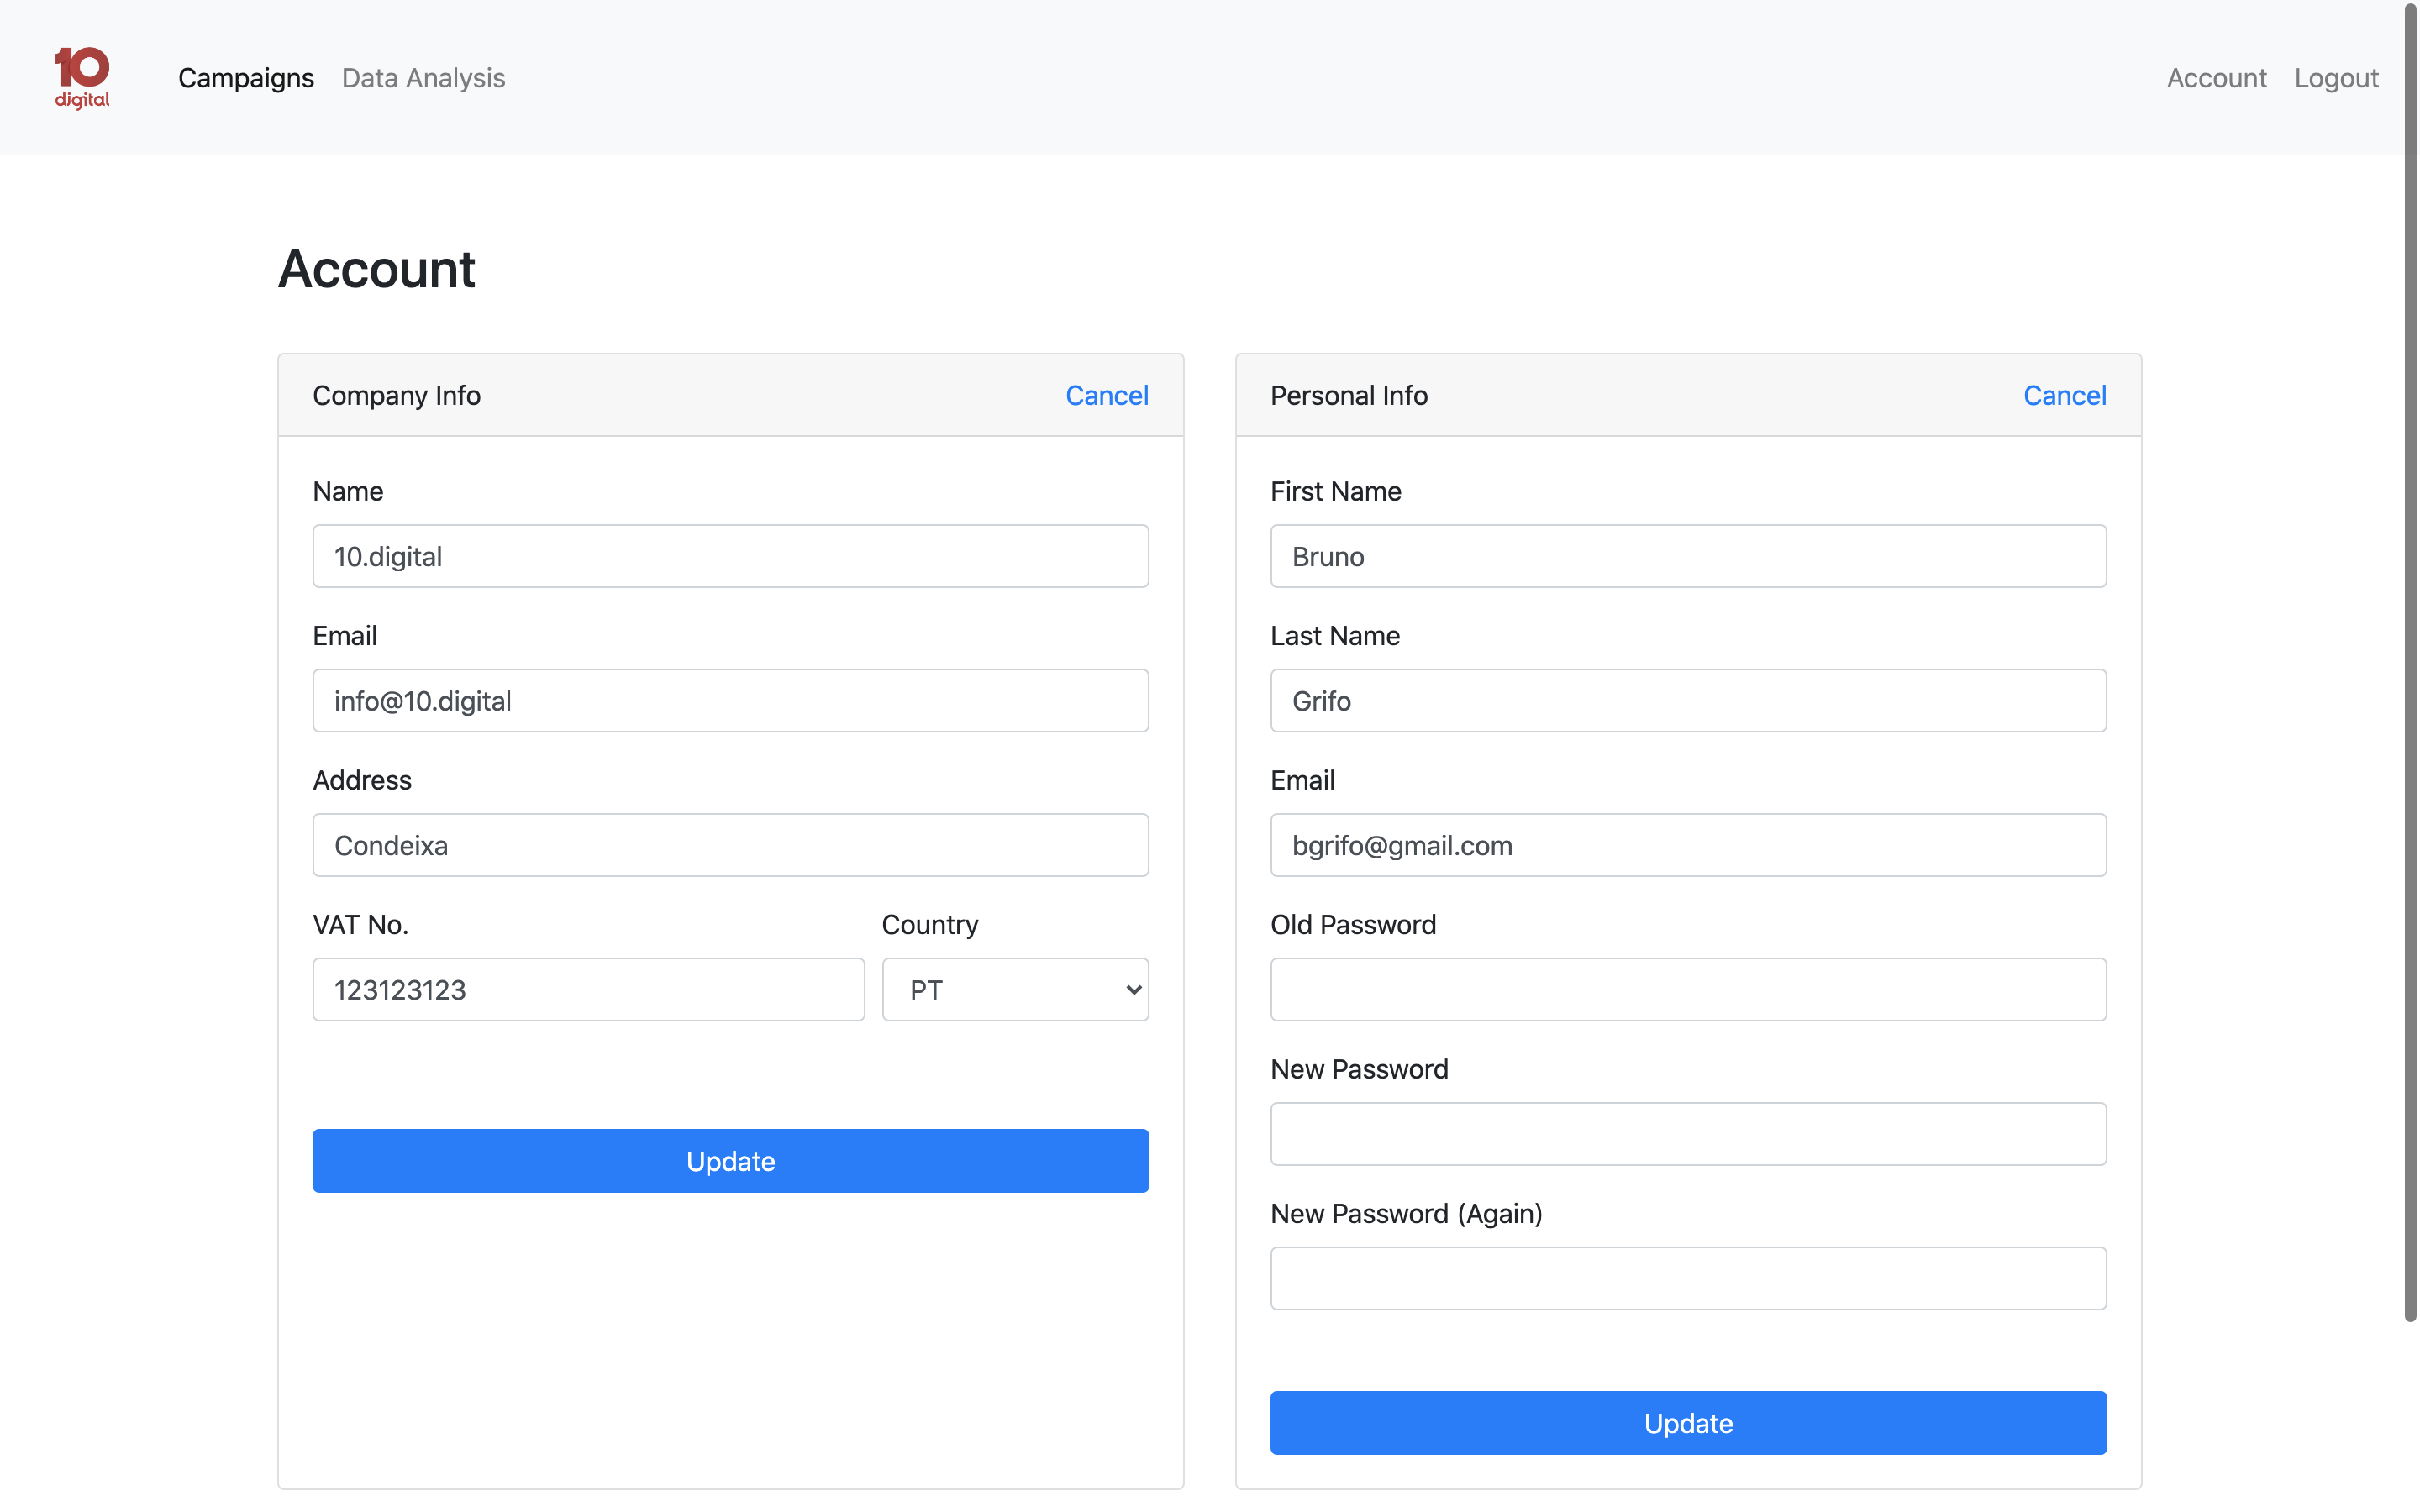
\includegraphics[width=0.8\textwidth]{img/product/account}
		\caption{10.quest - Definições de Conta}
		\label{fig:account}
	\end{center}
\end{figure}

\newpage


Ao entrar na página principal pode-se observar a lista de campanhas, separadas por tipos (i. e. questionários de personalidade e formações), tal como se verifica na Figura \ref{fig:home}. As listas de campanhas mostram também alguns detalhes associados às mesmas como o estado e a data de fim.

Para criar um questionário de personalidade basta carregar no botão que diz "New Personality Quiz" e para editar, basta selecionar um dos questionários de personalidade. Como se pode verificar na Figura \ref{fig:pq} para criar/editar uma campanha do tipo questionário de personalidade, é necessário introduzir um nome, descripção (opcional), data de fim, hora de fim e uma ou mais tags.

\begin{figure}[ht!]
	\begin{center}
		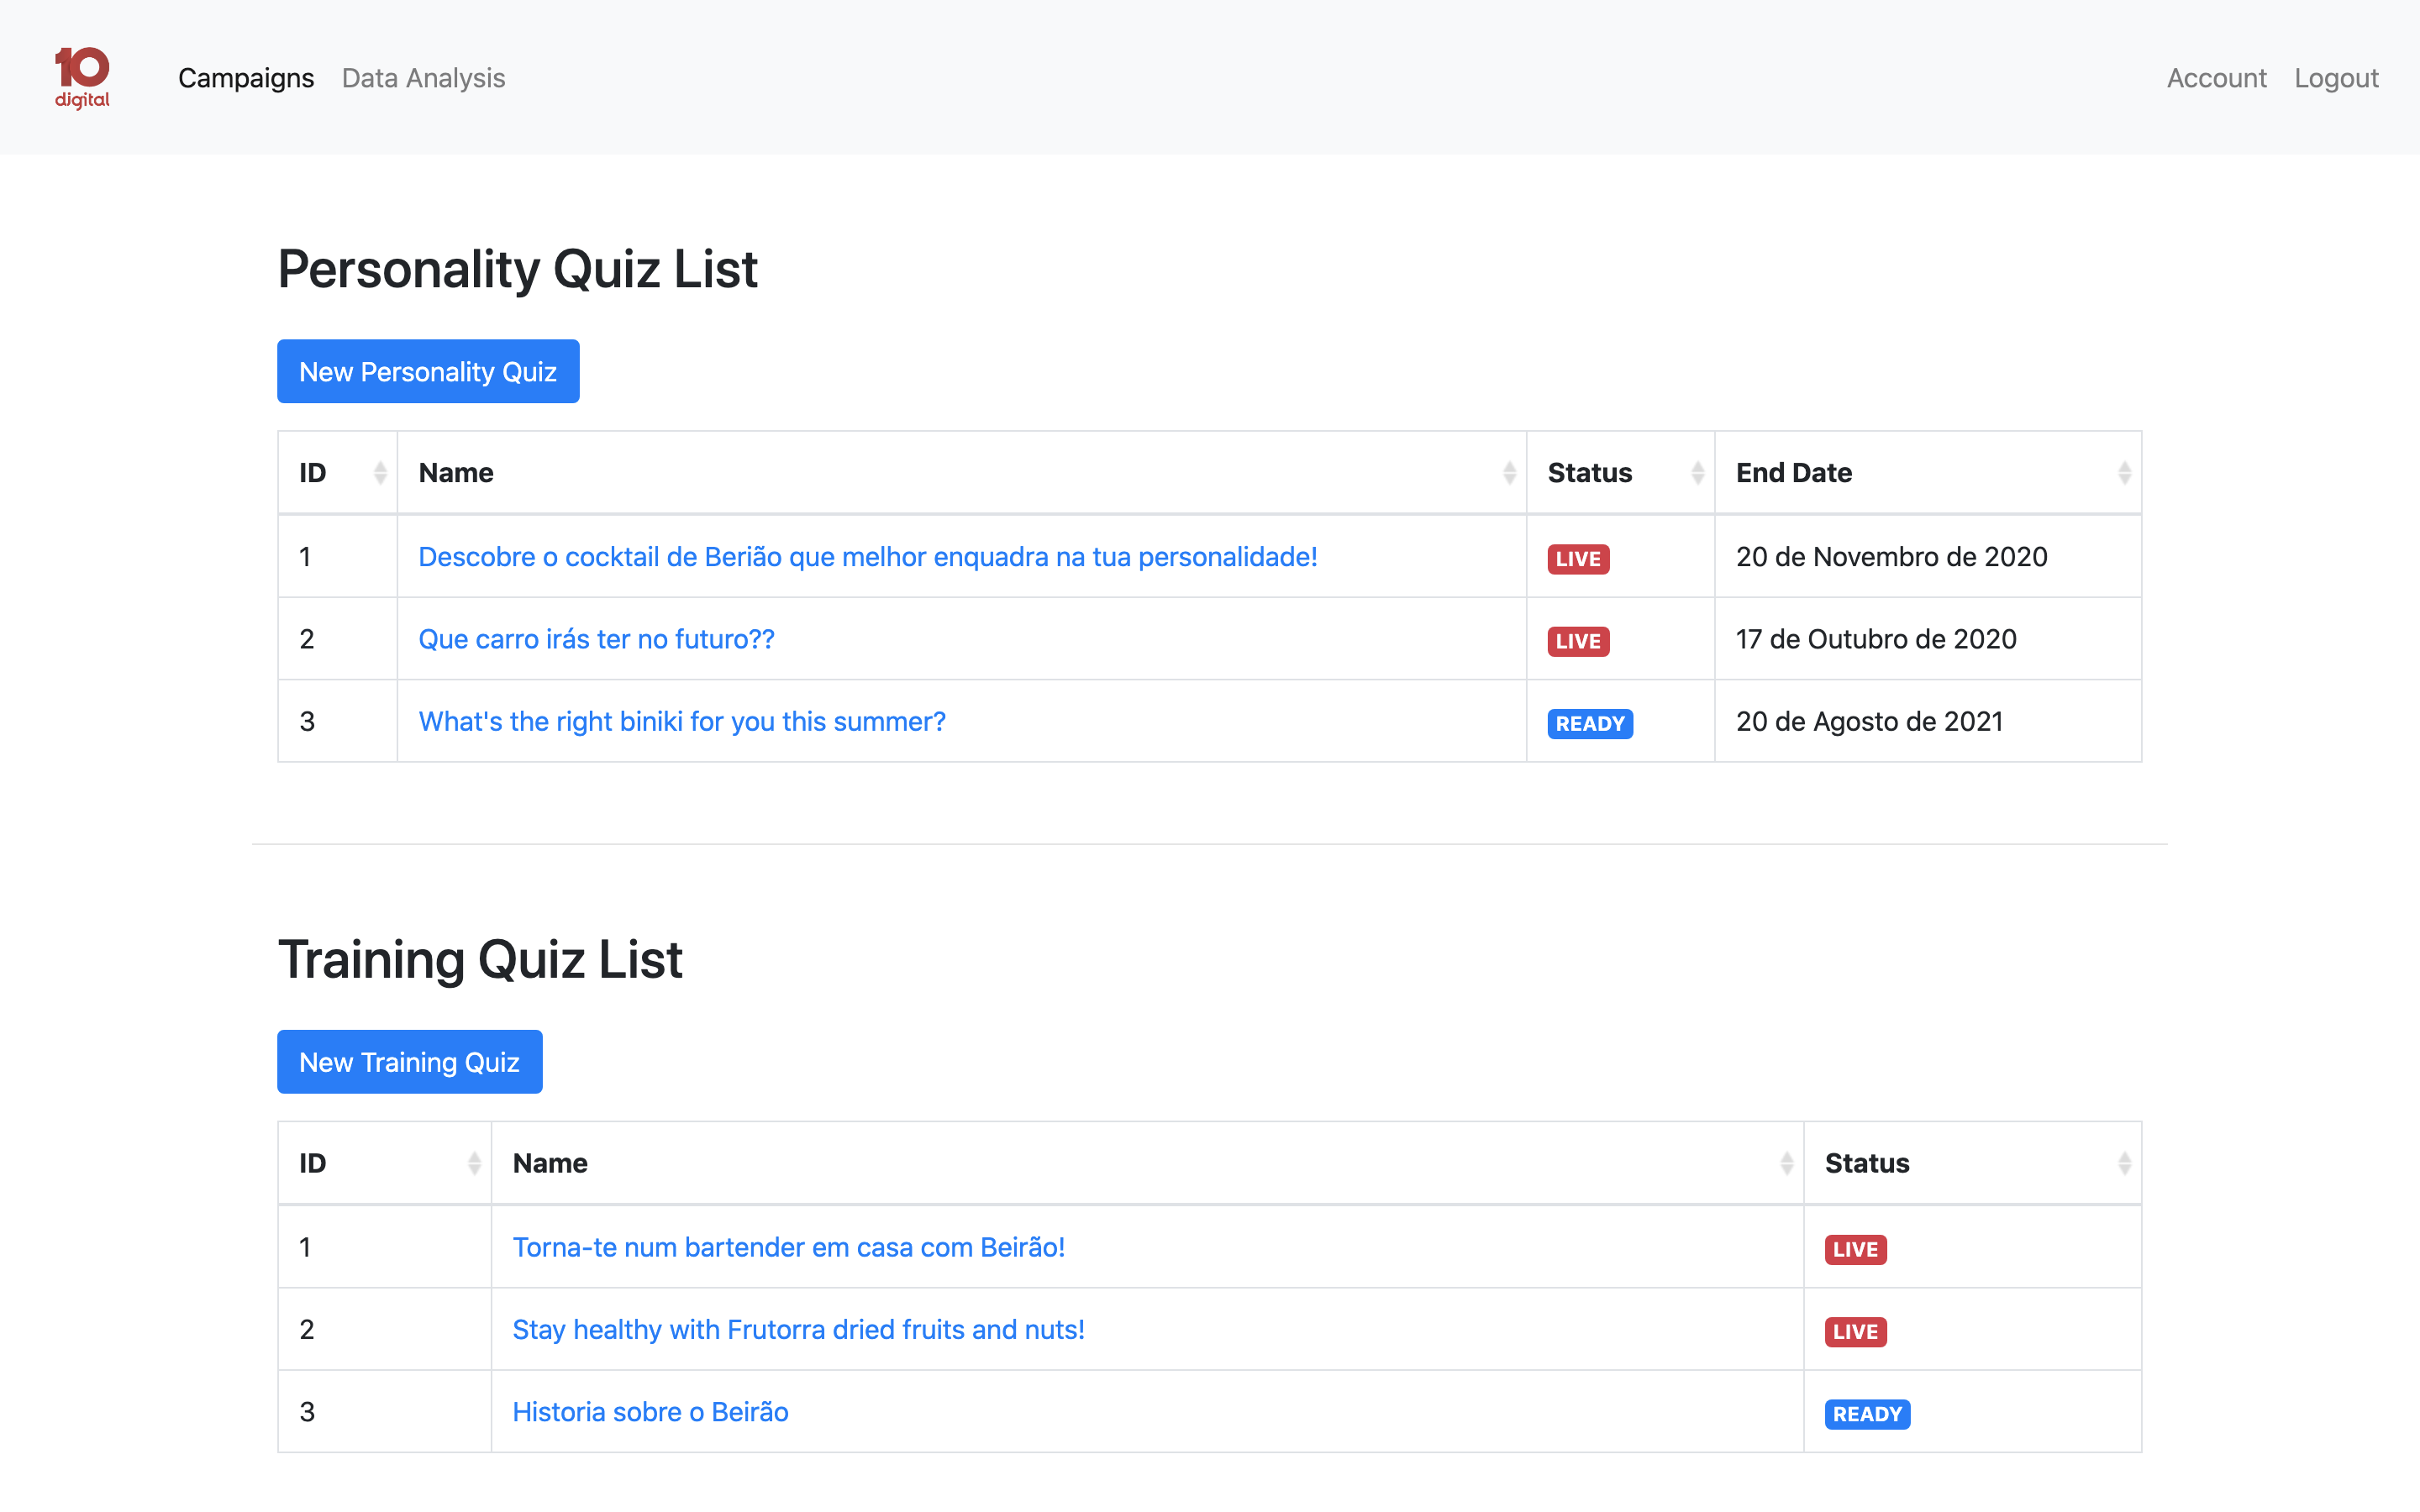
\includegraphics[width=0.8\textwidth]{img/product/homepage}
		\caption{10.quest - Página principal}
		\label{fig:home}
	\end{center}
\end{figure}

\begin{figure}[ht!]
	\begin{center}
		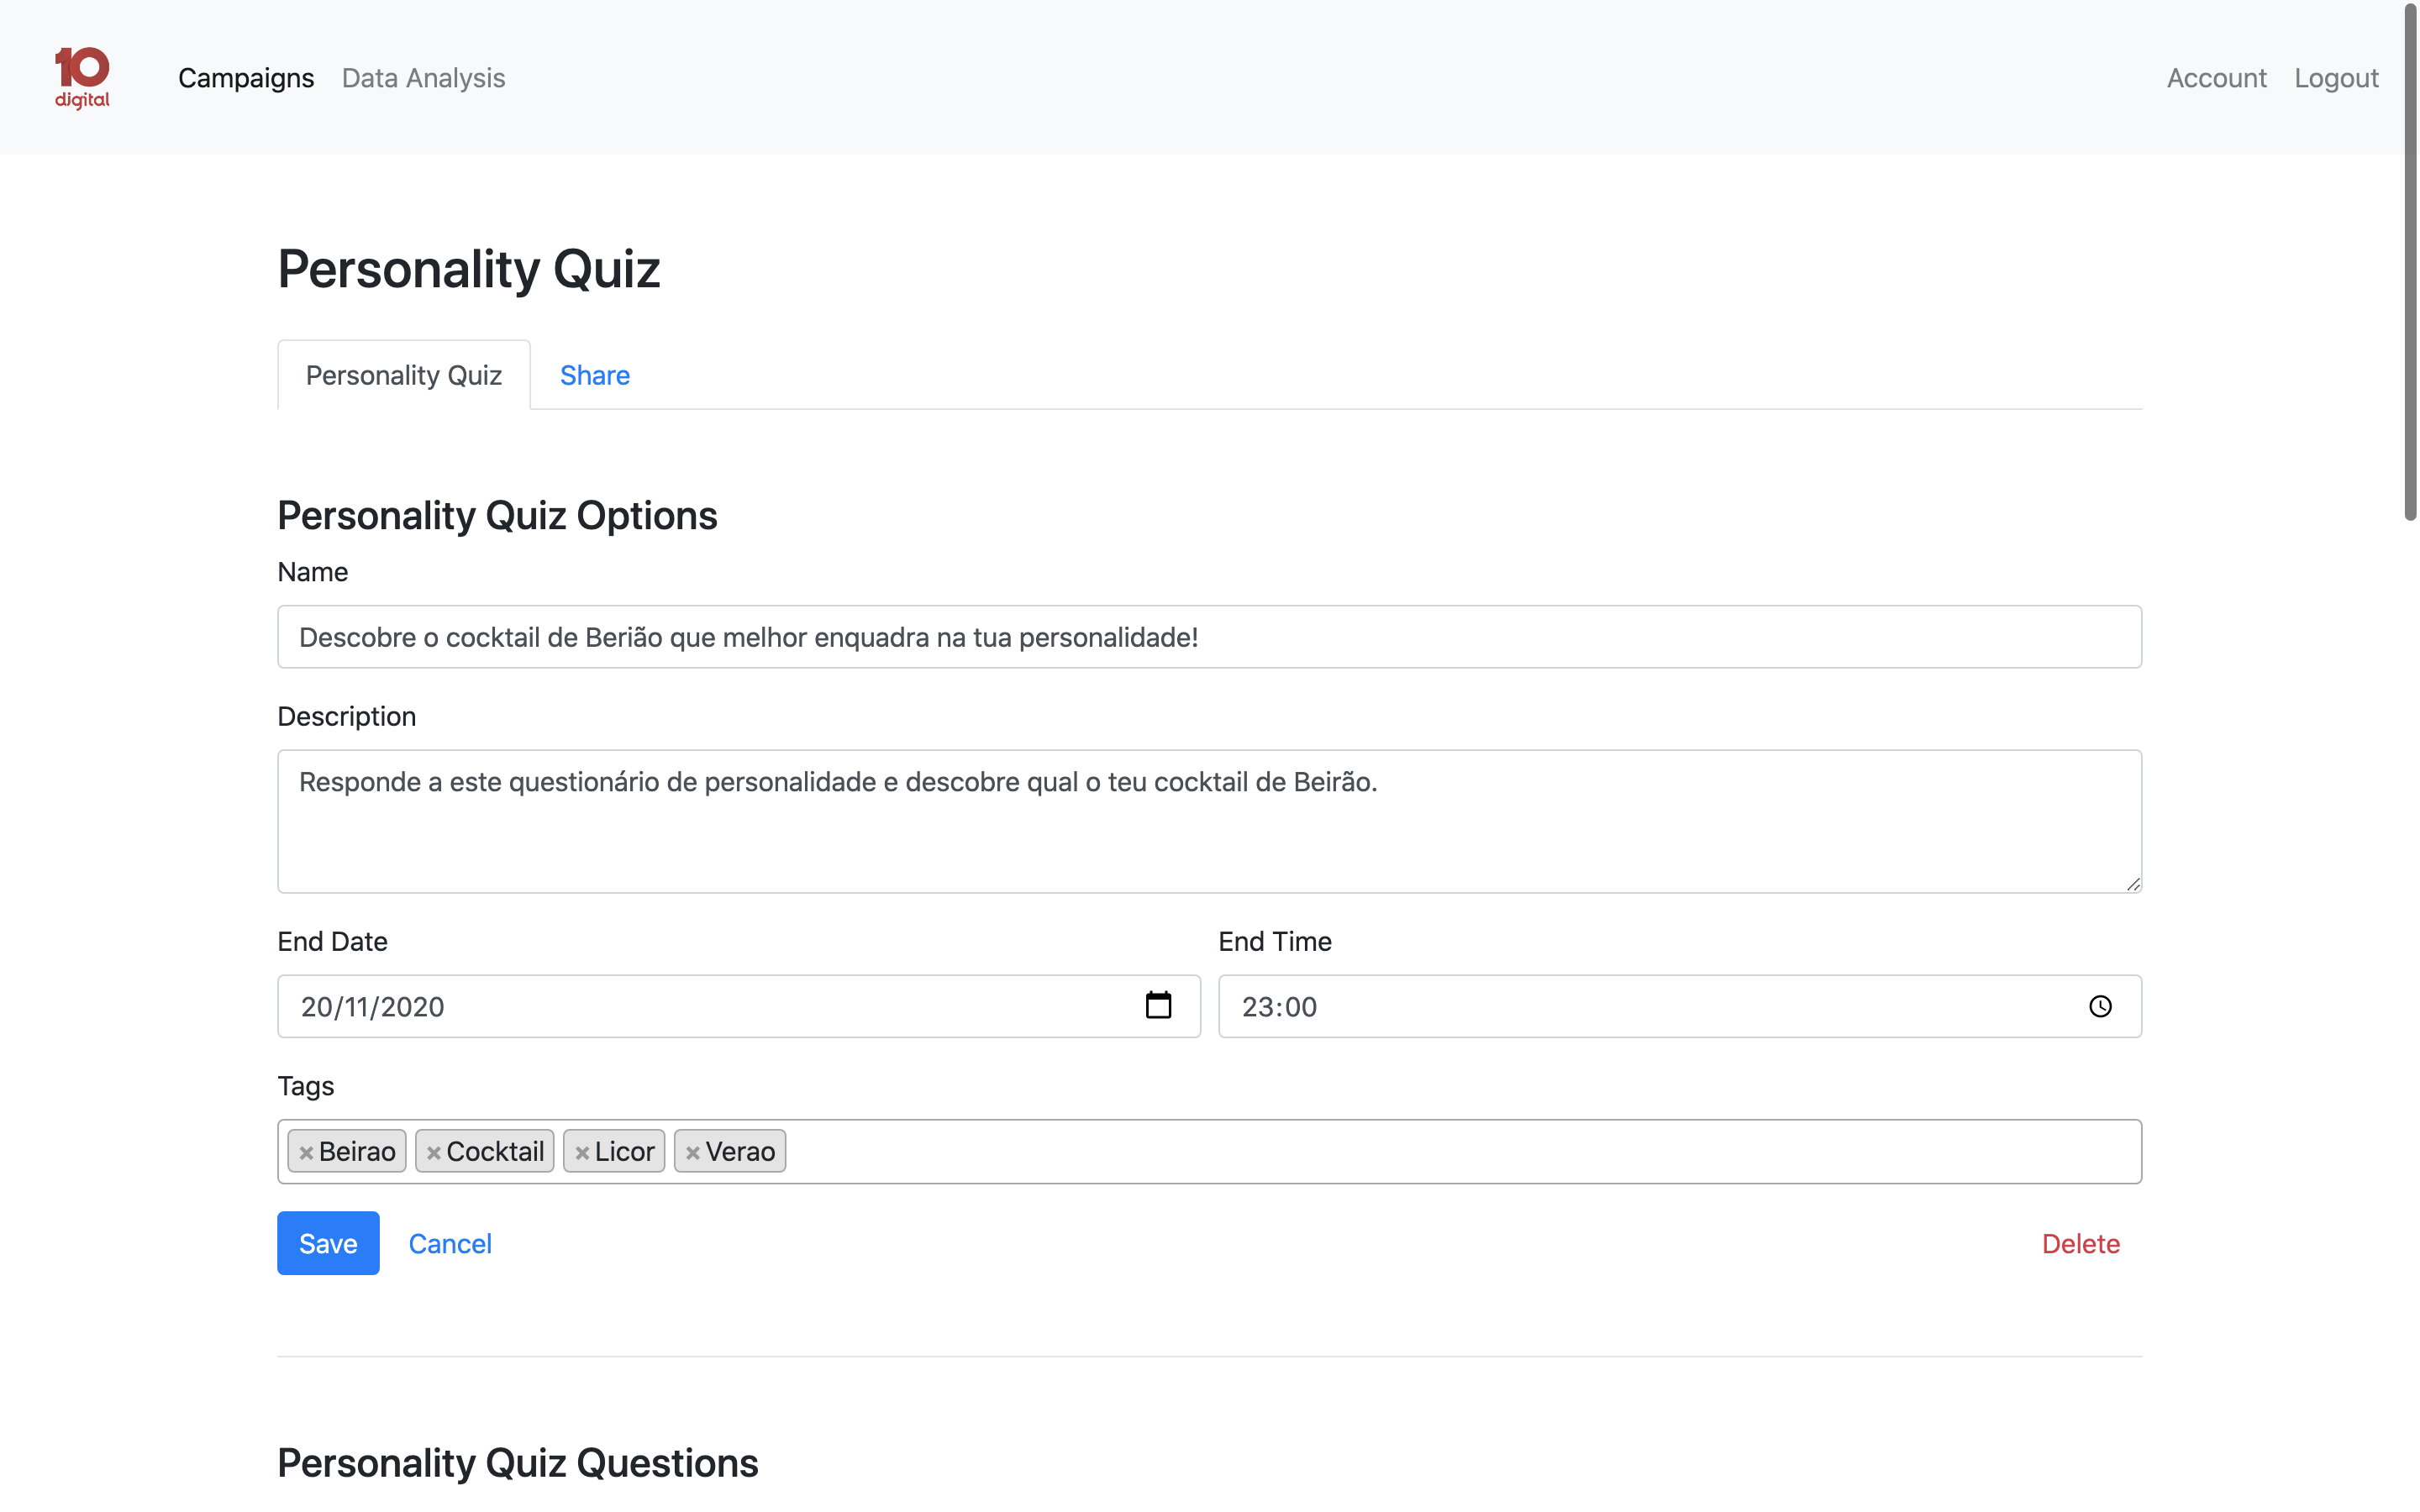
\includegraphics[width=0.8\textwidth]{img/product/pq}
		\caption{10.quest - Criar/Editar Questionário de Personalidade}
		\label{fig:pq}
	\end{center}
\end{figure}
\newpage



\begin{figure}[ht!]
	\begin{center}
		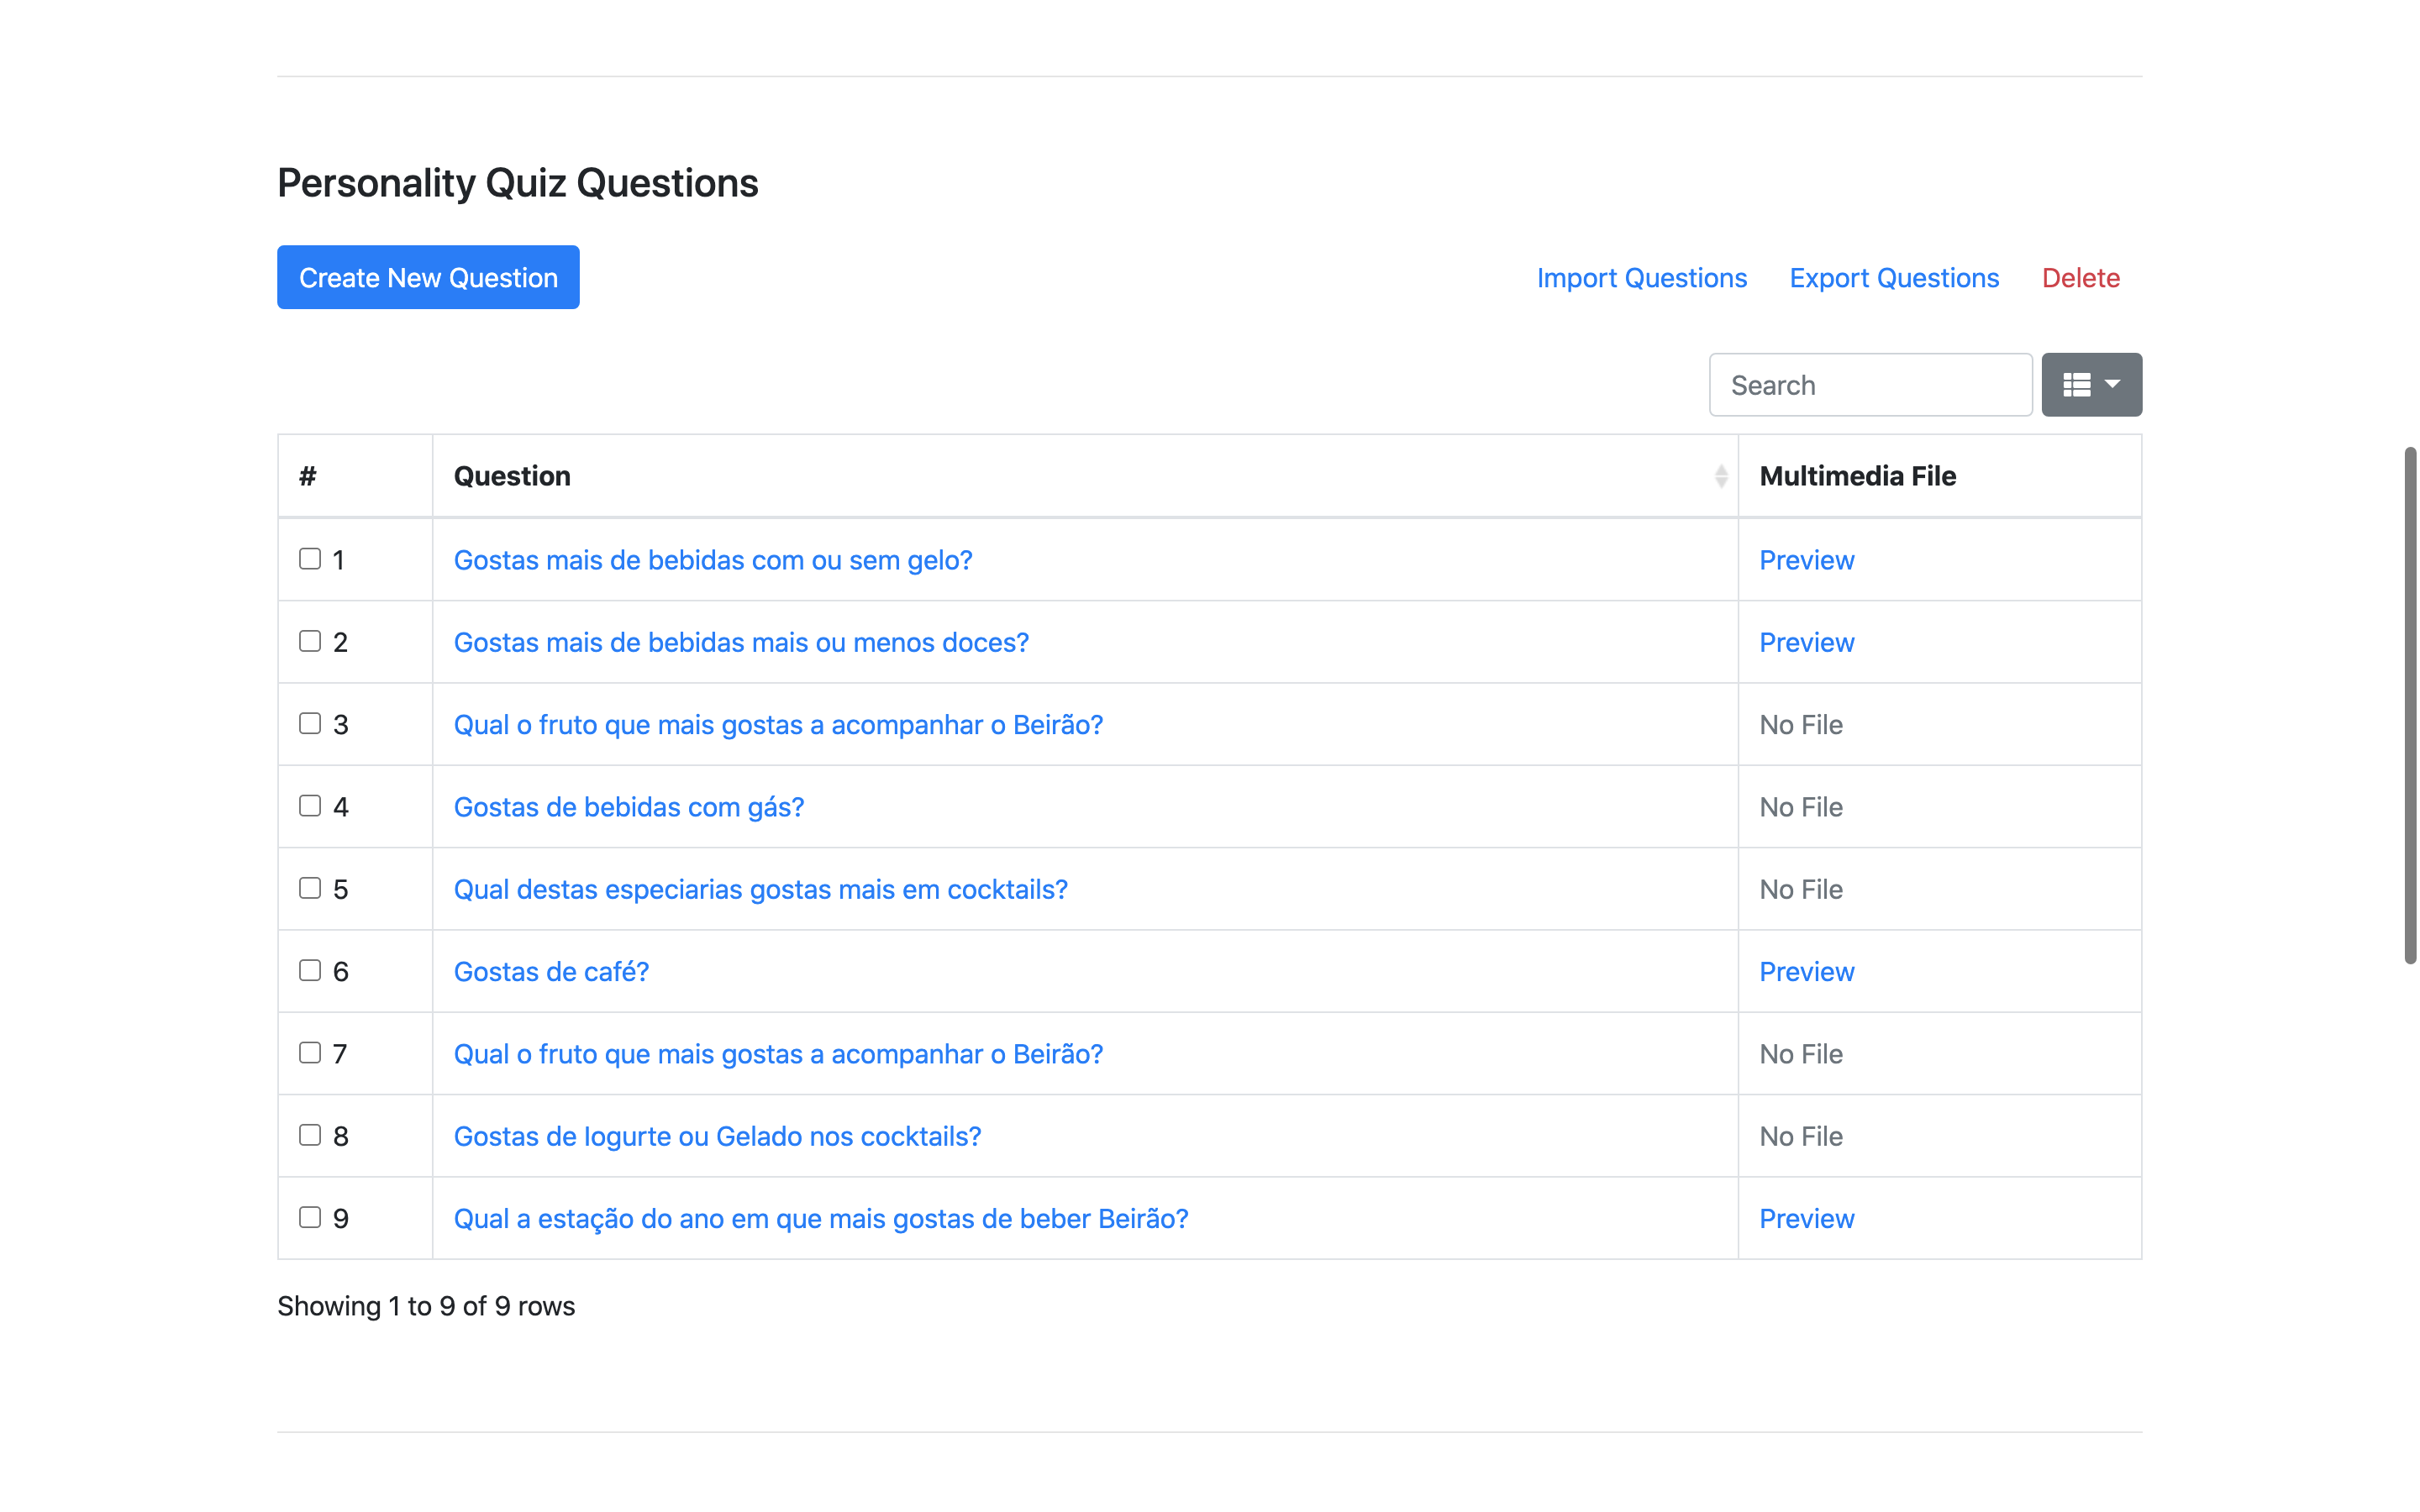
\includegraphics[width=0.8\textwidth]{img/product/pq_questions}
		\caption{10.quest - Lista de questões do Questionário de Personalidade}
		\label{fig:pq_questions}
	\end{center}
\end{figure}


\begin{figure}[ht!]
	\begin{center}
		\begin{minipage}{0.45\textwidth}
			\begin{center}
				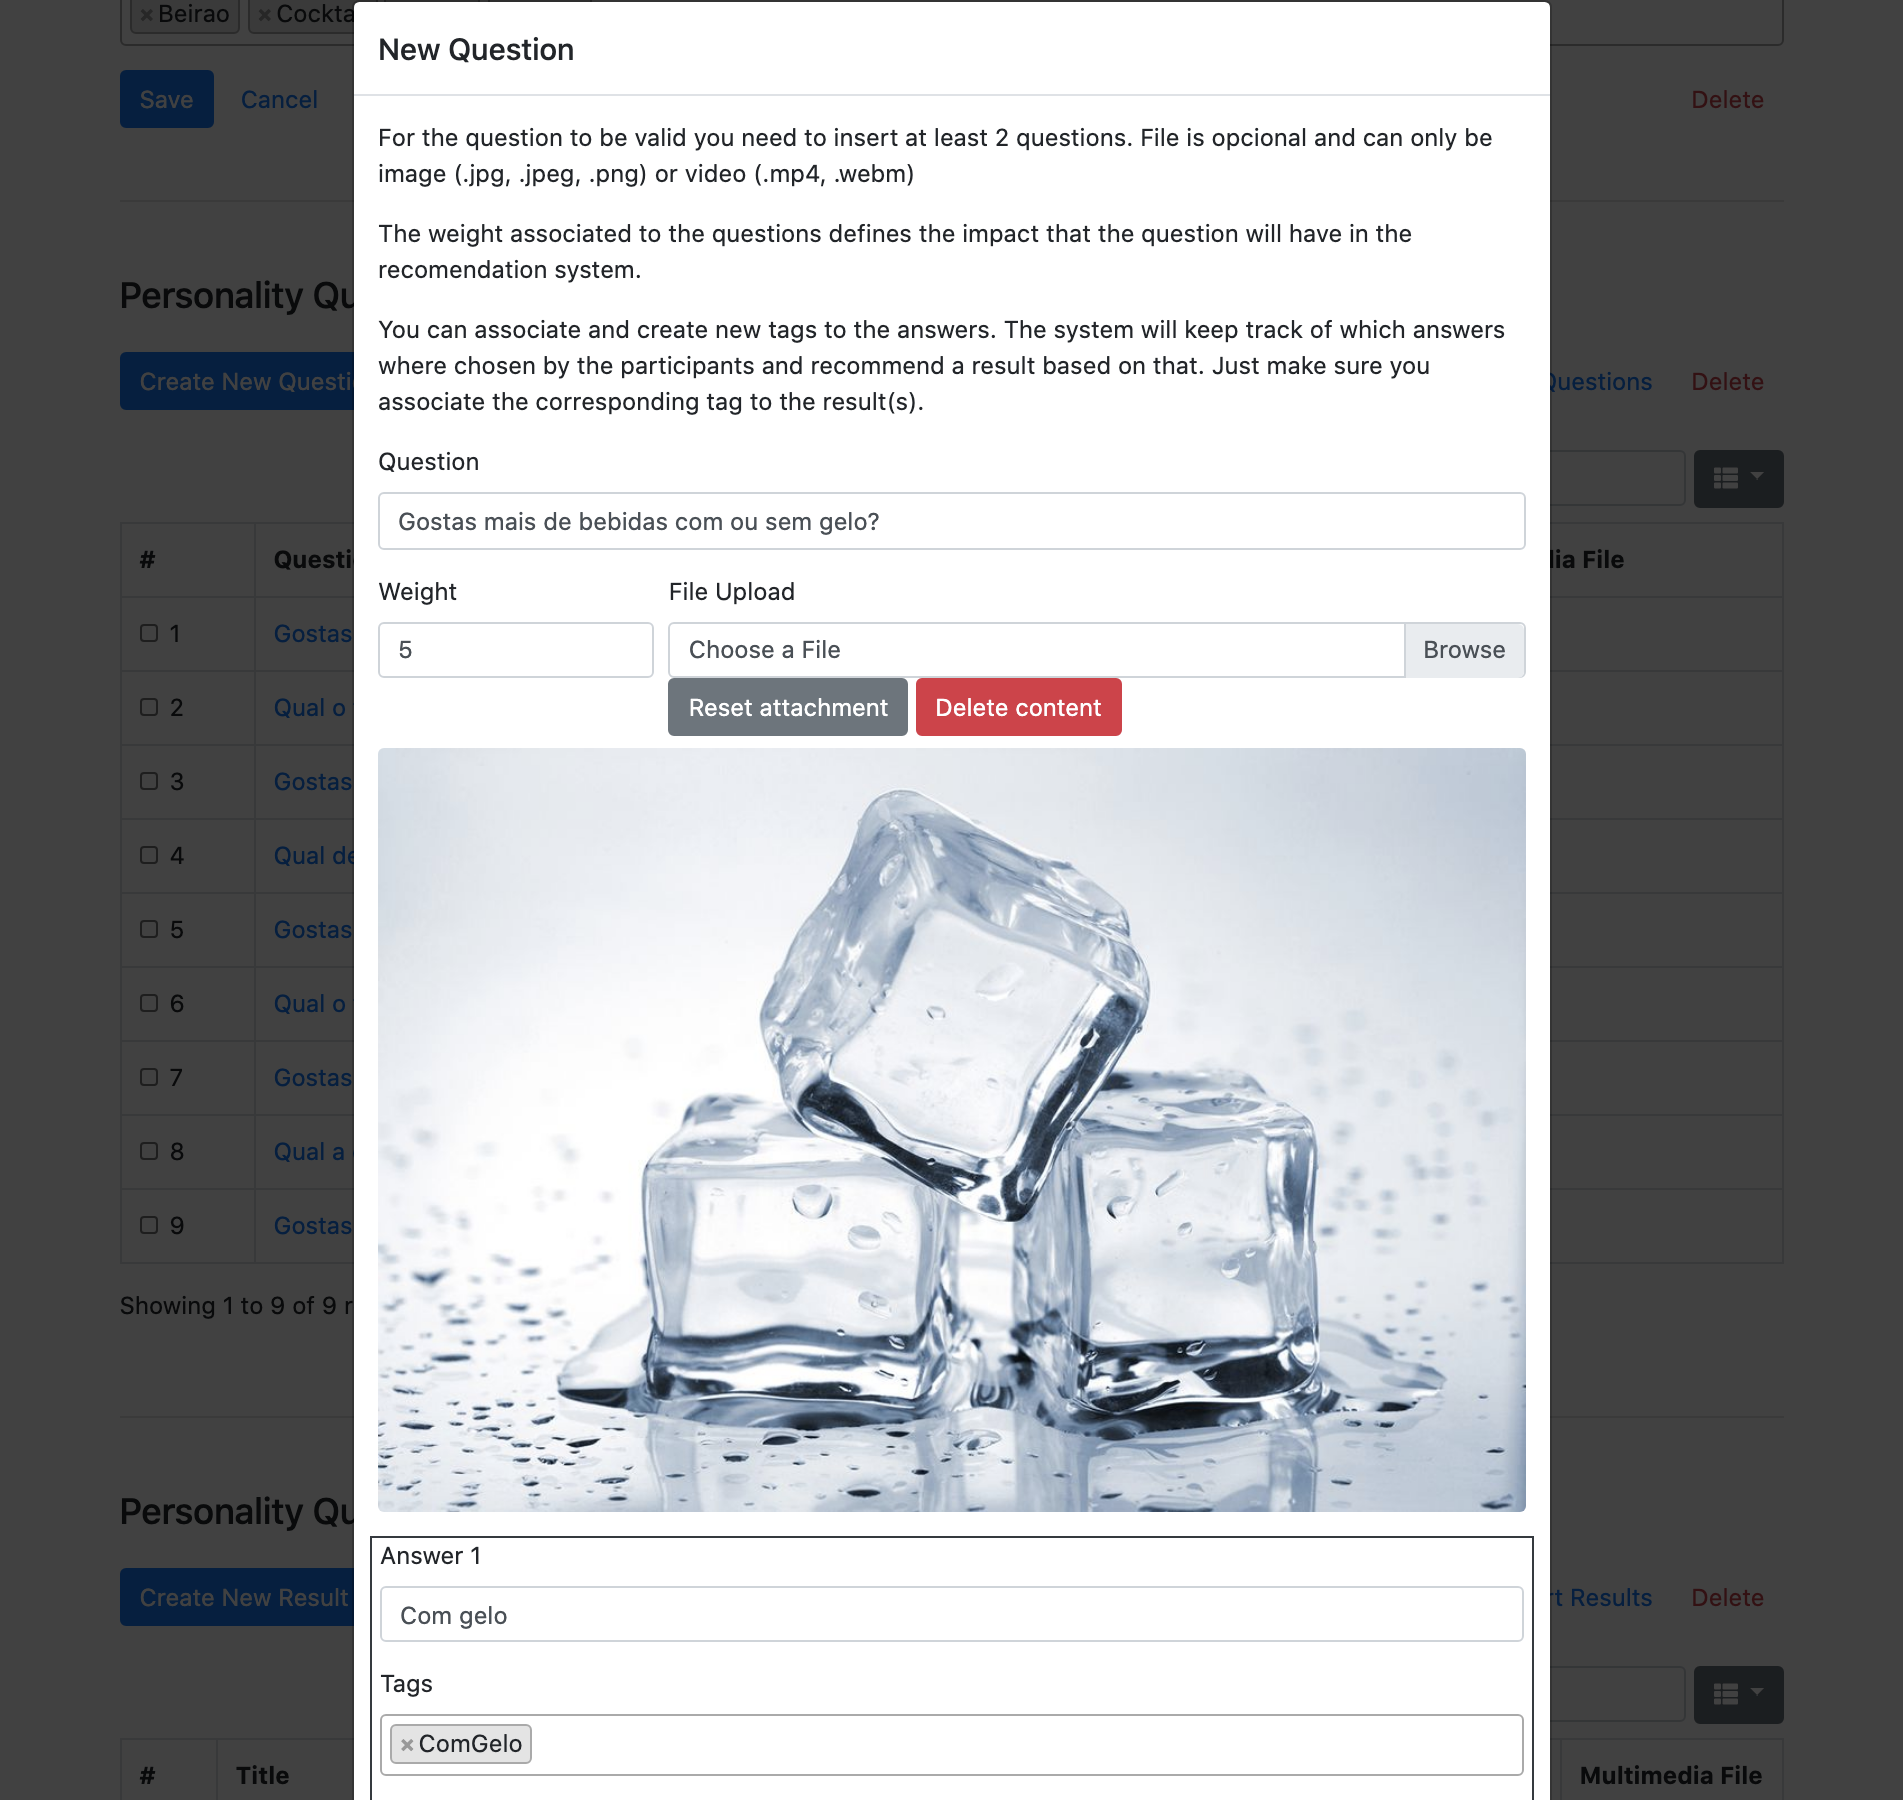
\includegraphics[height=.3\textheight]{img/product/pq_q1}
				\caption{10.quest - Criar/Editar uma questão}
				\label{fig:pq_q1}
			\end{center}
		\end{minipage}
		\hspace{1cm}
		\begin{minipage}{0.45\textwidth}
			\begin{center}
				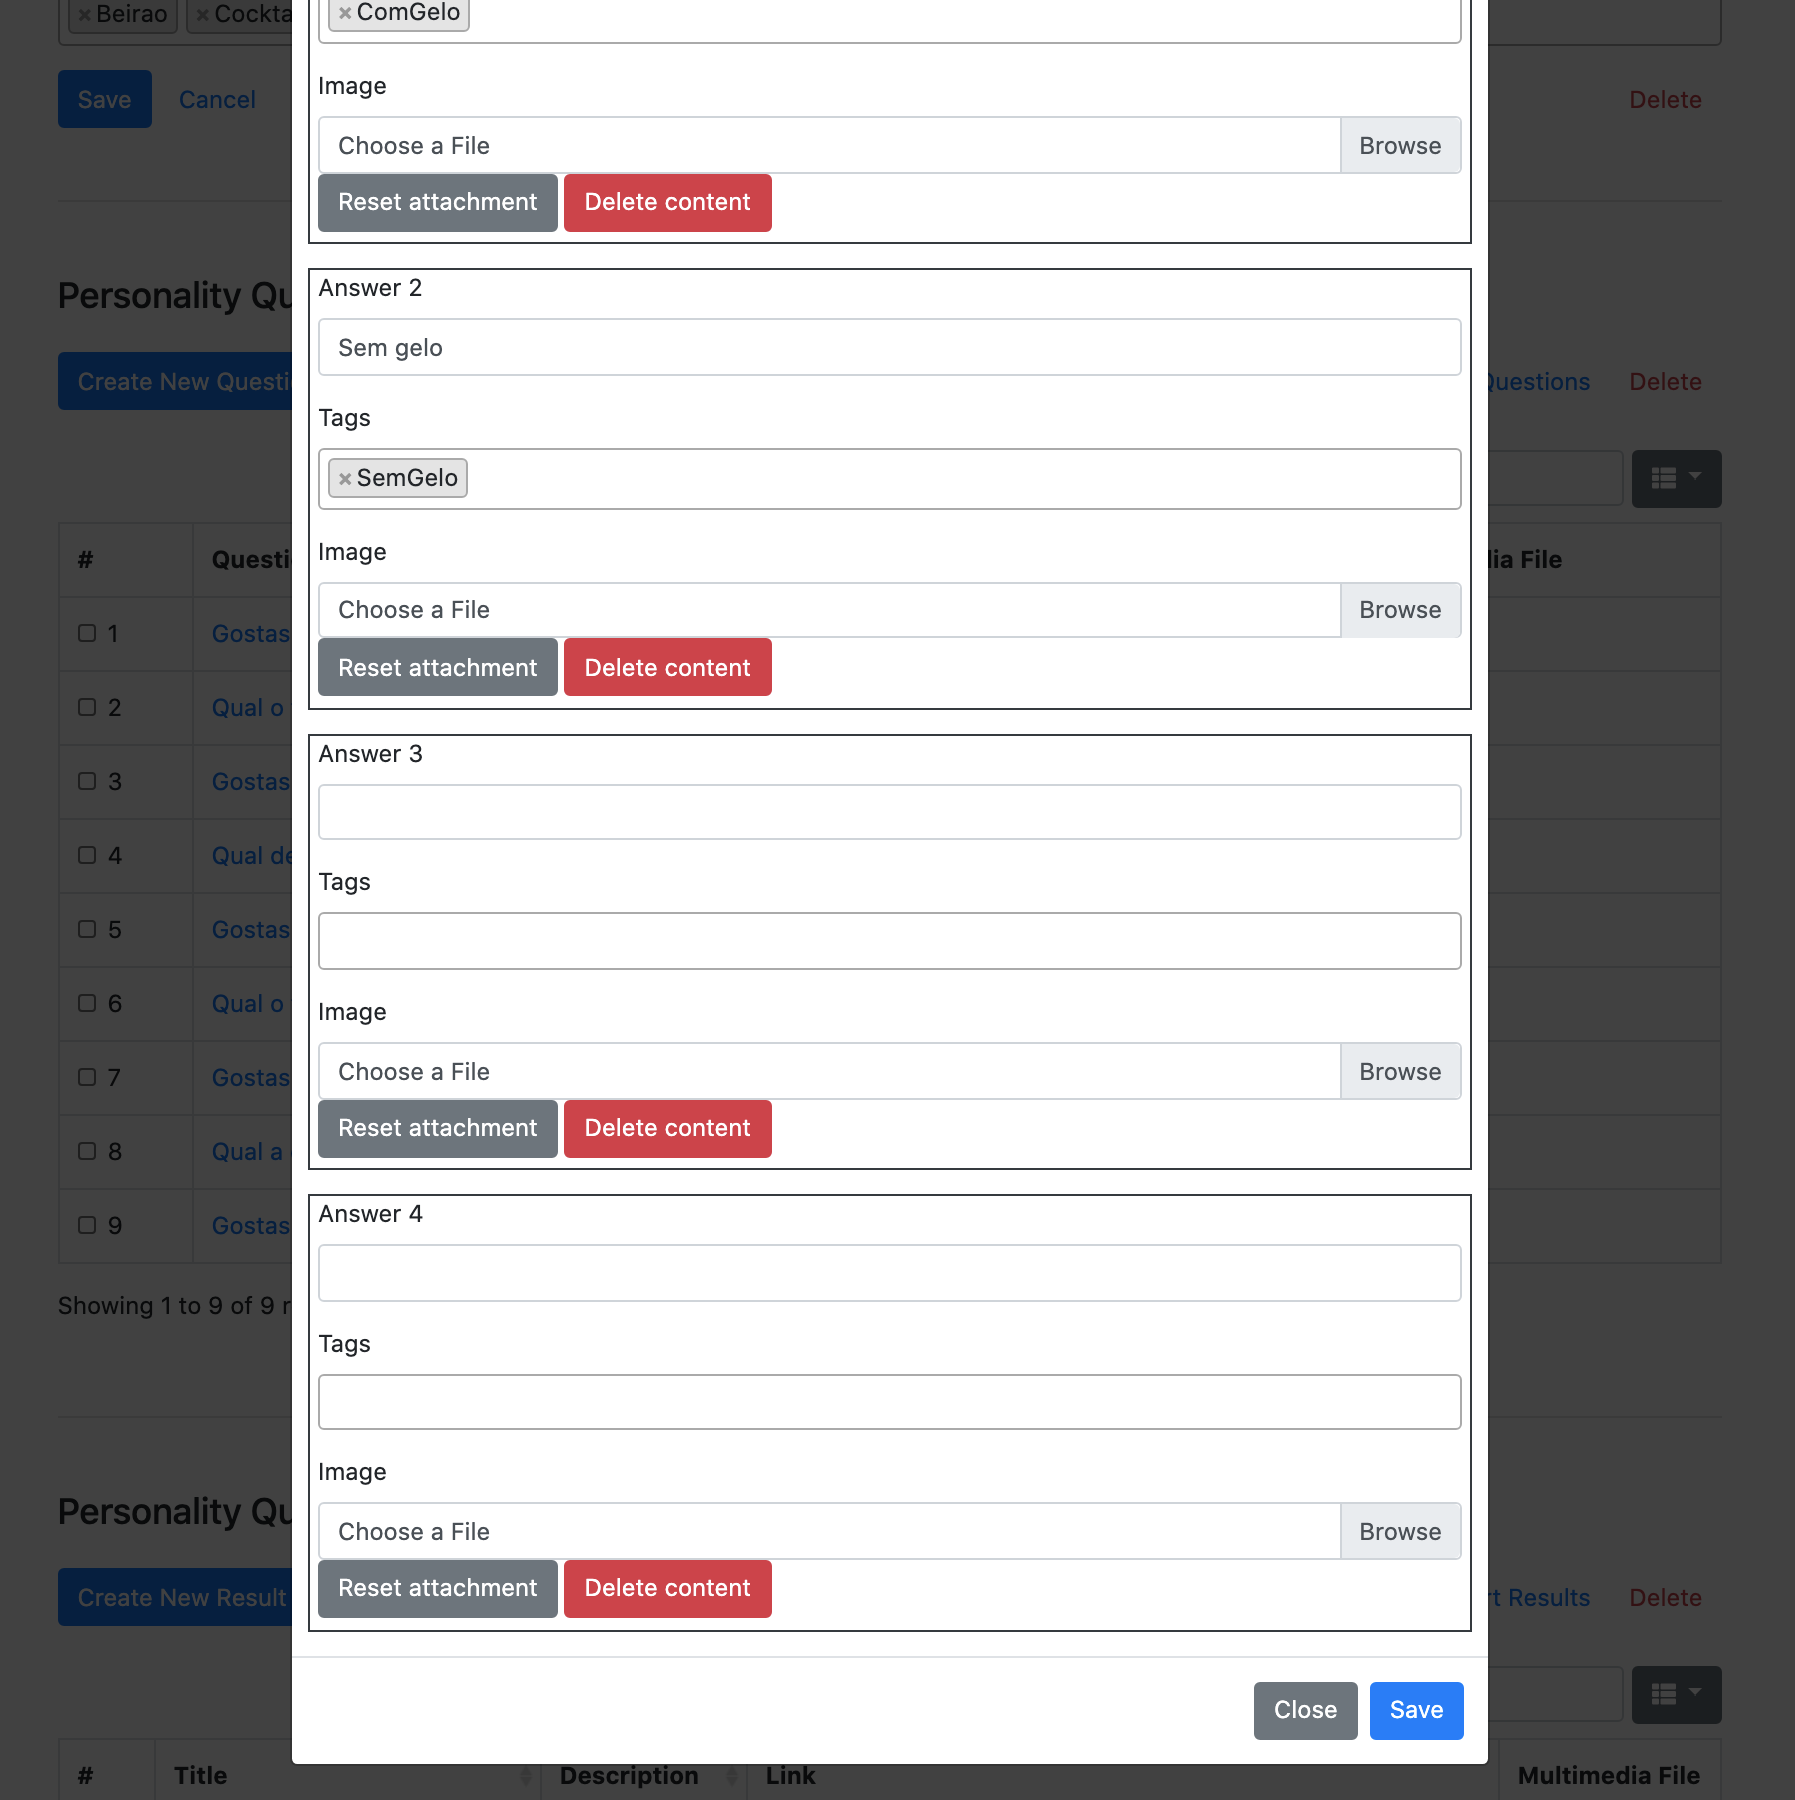
\includegraphics[height=.3\textheight]{img/product/pq_q2}
				\caption{10.quest - Criar/Editar uma questão}
				\label{fig:pq_q2}
			\end{center}
		\end{minipage}
	\end{center}
\end{figure}

\begin{figure}[ht!]
	\begin{center}
		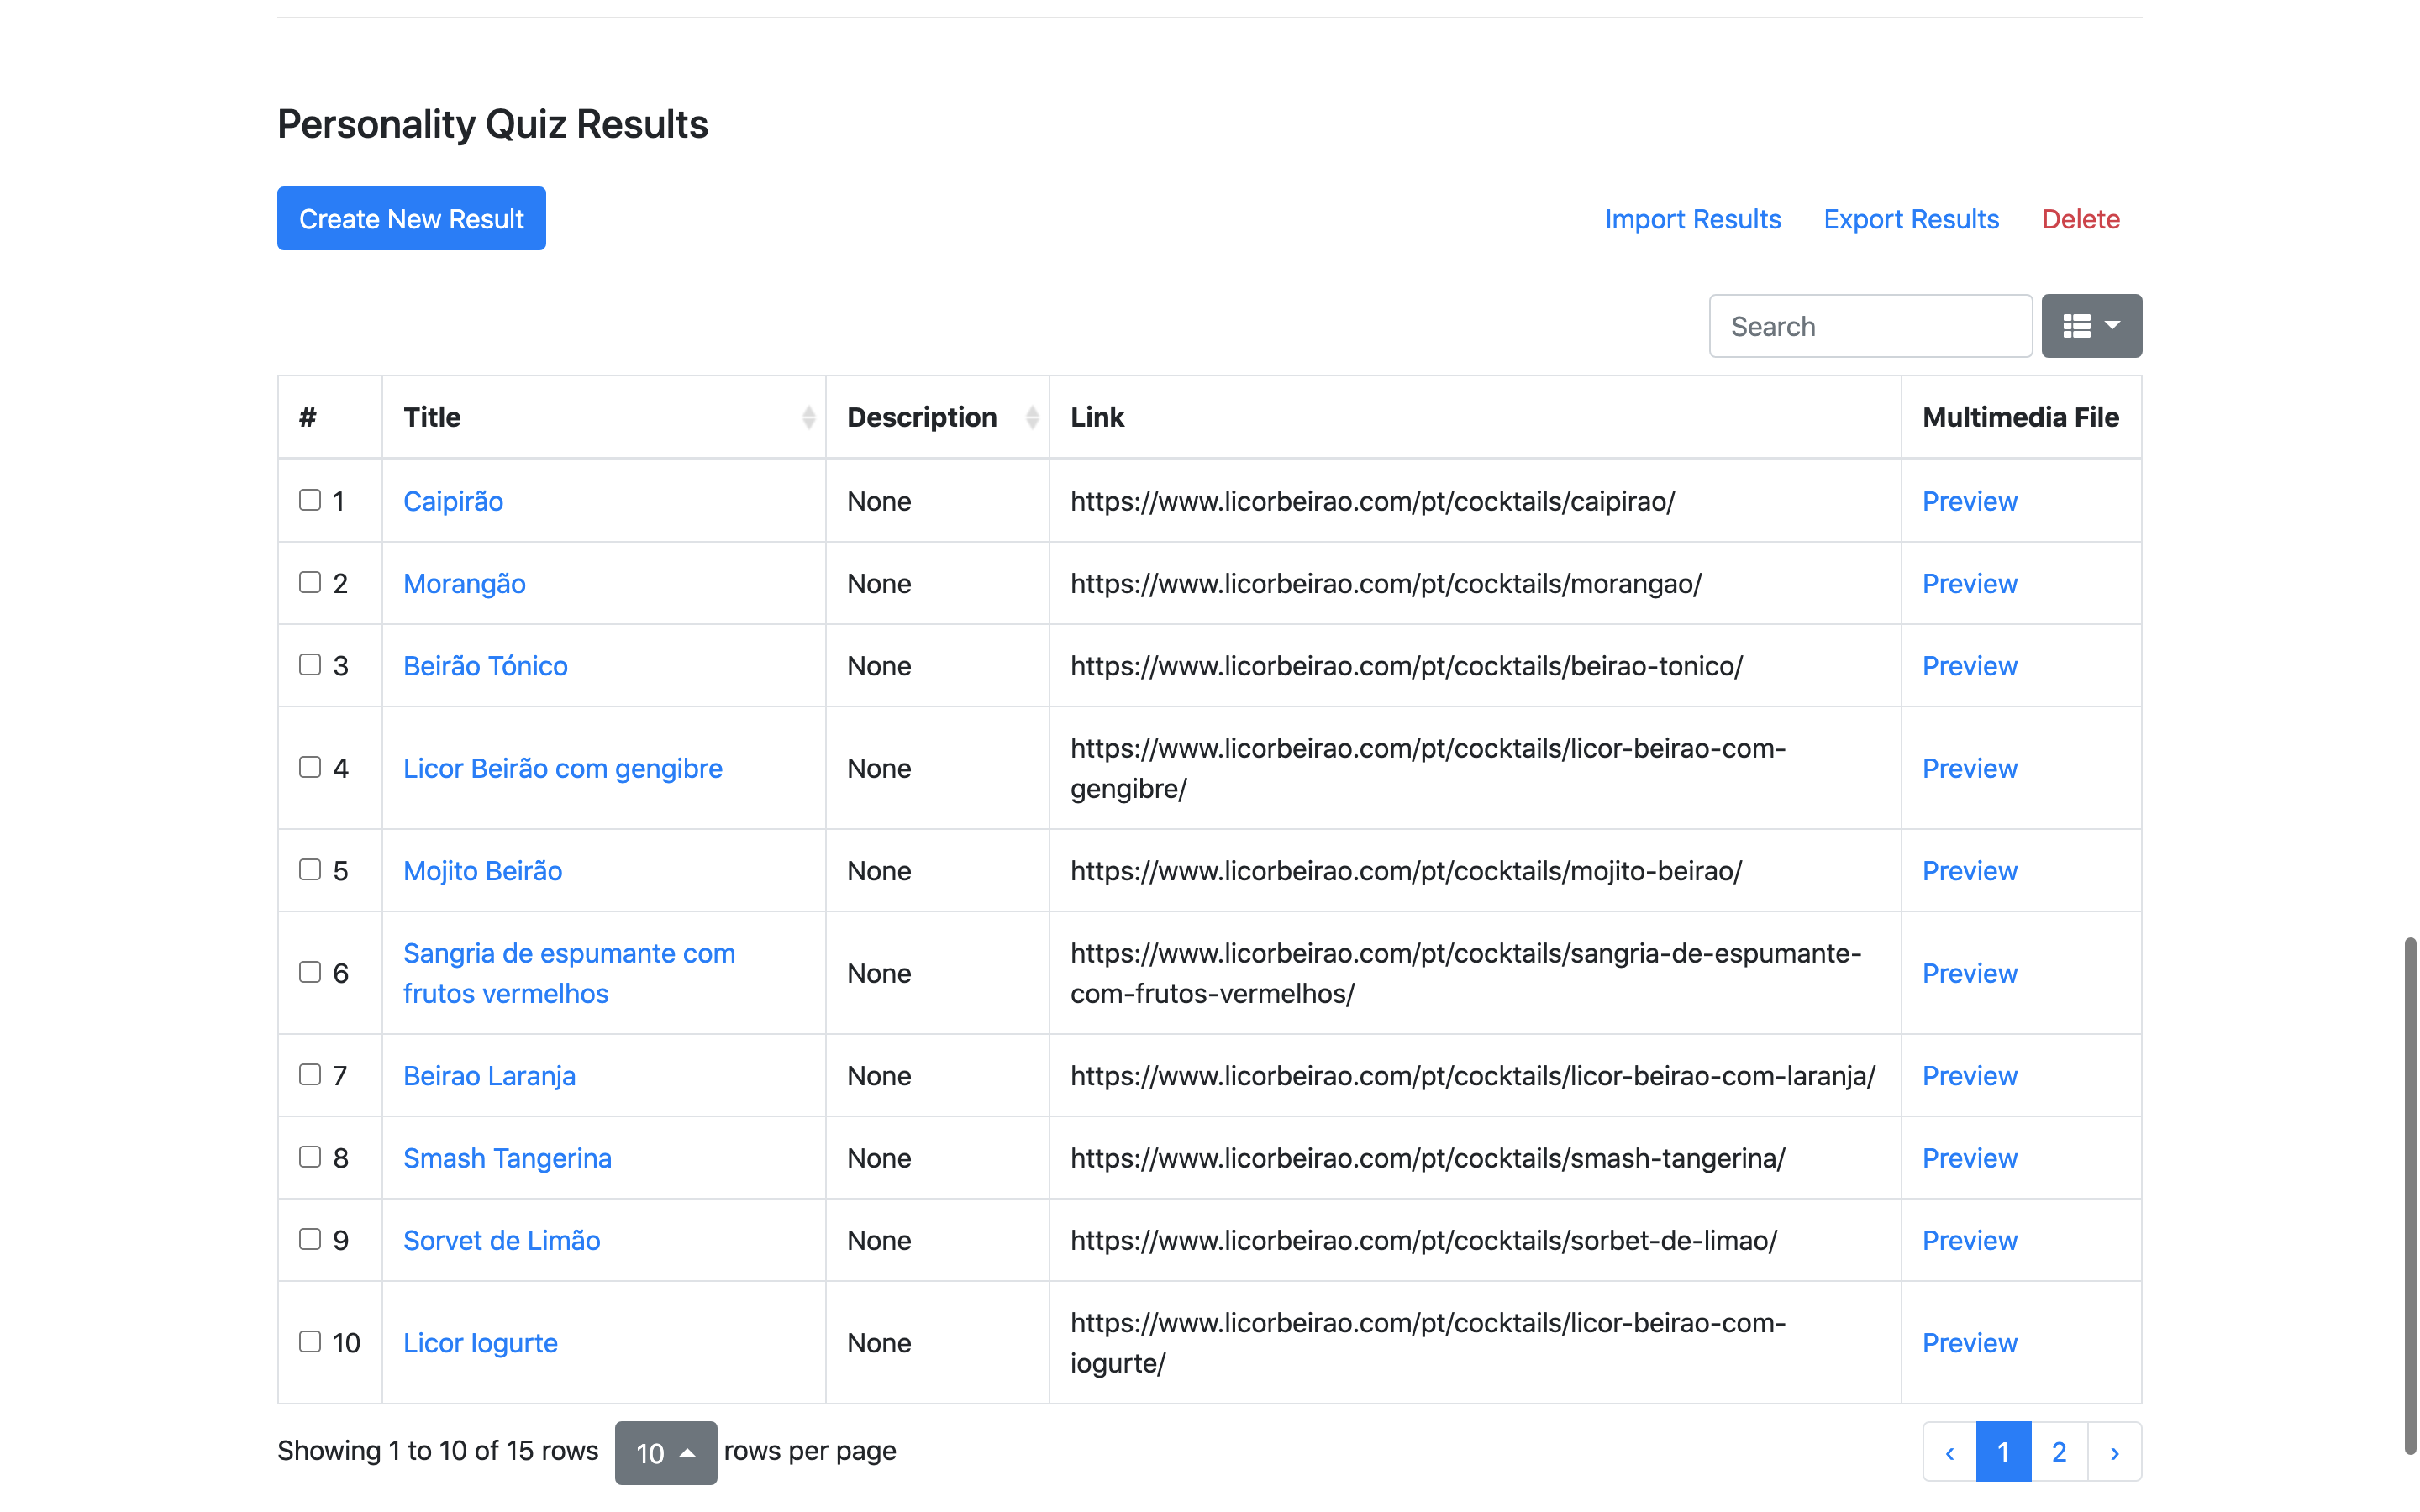
\includegraphics[width=0.8\textwidth]{img/product/pq_results}
		\caption{10.quest - Lista de resultados do Questionário de Personalidade}
		\label{fig:pq_results}
	\end{center}
\end{figure}

\begin{figure}[ht!]
	\begin{center}
		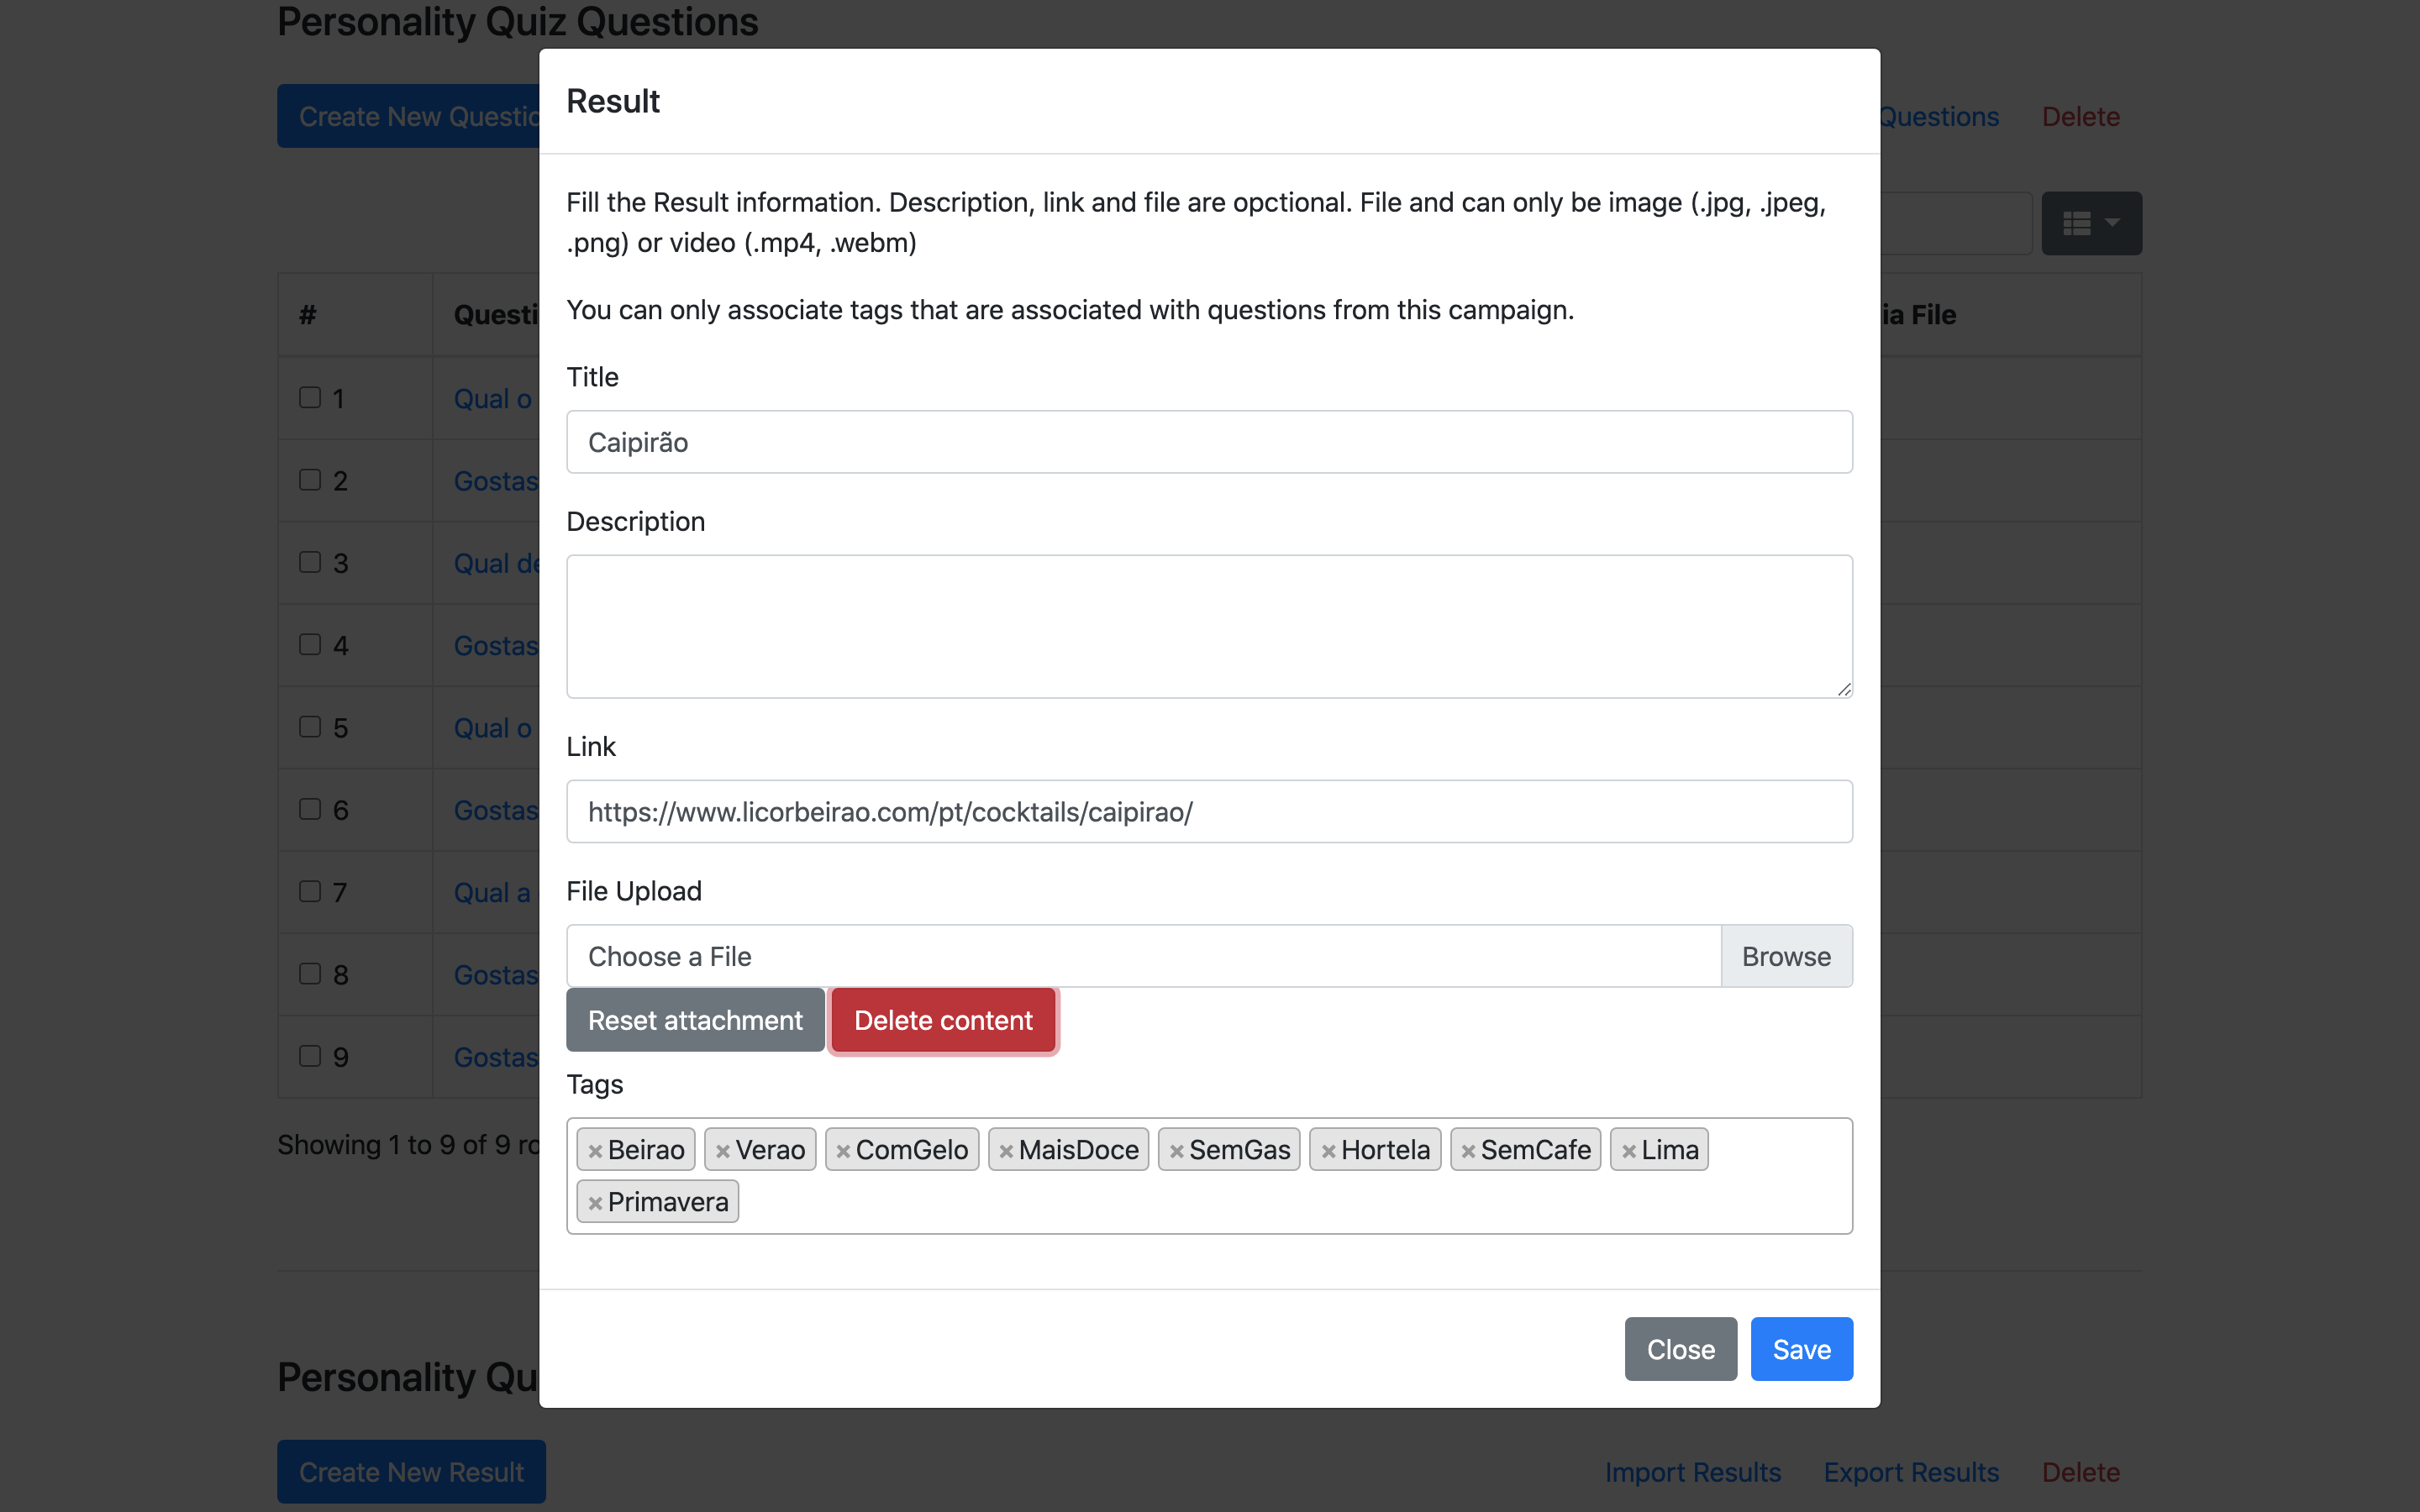
\includegraphics[width=0.8\textwidth]{img/product/pq_result}
		\caption{10.quest - Criar/Editar um resultado}
		\label{fig:pq_result}
	\end{center}
\end{figure}



\section{Trabalho Futuro}

%-------------------------------------------------------------------------------------------------
\blankpage
%-------------------------------------------------------------------------------------------------

\glsresetall
